\documentclass{standalone}
\usepackage{tikz}
\begin{document}
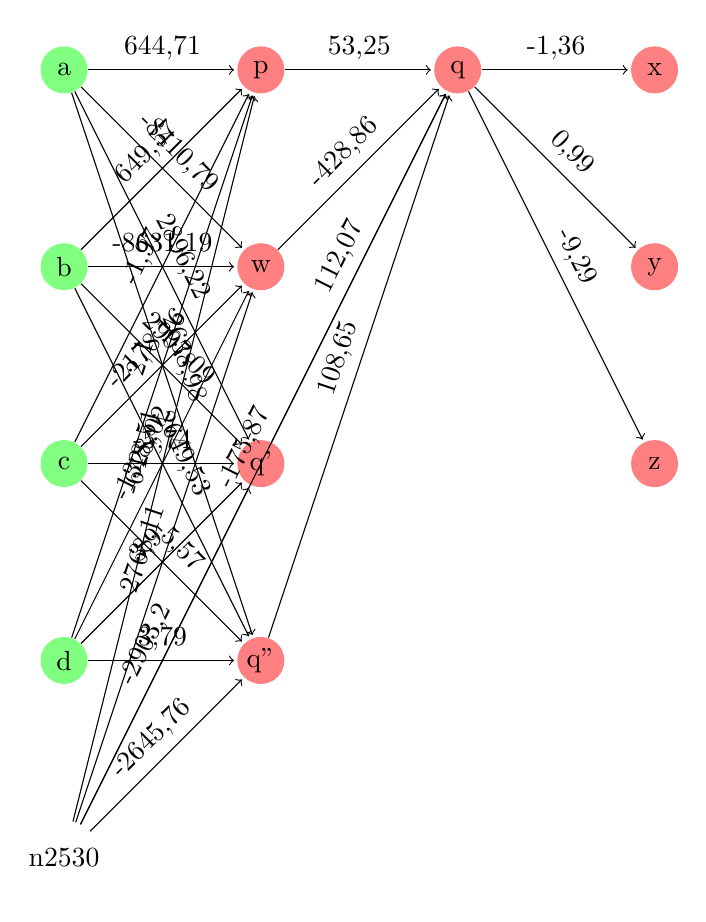
\begin{tikzpicture}[shorten >=1pt,->,draw=black!,node distance=2.5cm]
\tikzstyle{neuron}=[circle,fill=black!25,minimum size=17pt,inner sep=0pt]
\tikzstyle{constant}=[neuron, fill=white!50];
\tikzstyle{sigmoid}=[neuron, fill=red!50];
\tikzstyle{identity}=[neuron, fill=green!50];
\node [identity] (a) {a};
\node [identity,below of=a] (b) {b};
\node [identity,below of=b] (c) {c};
\node [identity,below of=c] (d) {d};
\node [constant,below of=d] (n2530) {n2530};
\node [sigmoid,right of=a] (p) {p};
\node [sigmoid,below of=p] (w) {w};
\node [sigmoid,below of=w] (q') {q'};
\node [sigmoid,below of=q'] (q'') {q''};
\node [sigmoid,right of=p] (q) {q};
\node [sigmoid,right of=q] (x) {x};
\node [sigmoid,below of=x] (y) {y};
\node [sigmoid,below of=y] (z) {z};
\path[every node/.style={sloped,anchor=south,auto=false}]
(n2530) edge node {2768,11} (w)
(n2530) edge node {-648,51} (p)
(n2530) edge node {-175,87} (q)
(n2530) edge node {-2645,76} (q'')
(n2530) edge node {-2903,2} (q')
(w) edge node {-428,86} (q)
(p) edge node {53,25} (q)
(q'') edge node {108,65} (q)
(q') edge node {112,07} (q)
(b) edge node {2907,09} (q')
(b) edge node {2649,53} (q'')
(b) edge node {649,57} (p)
(b) edge node {-8631,19} (w)
(a) edge node {2638,98} (q'')
(a) edge node {-8410,79} (w)
(a) edge node {2896,22} (q')
(a) edge node {644,71} (p)
(q) edge node {-9,29} (z)
(q) edge node {0,99} (y)
(q) edge node {-1,36} (x)
(d) edge node {3,9} (q')
(d) edge node {3,79} (q'')
(d) edge node {2,1} (p)
(d) edge node {-1328,02} (w)
(c) edge node {-5,57} (q'')
(c) edge node {-2178,16} (w)
(c) edge node {-5,74} (q')
(c) edge node {-1,97} (p)
;\end{tikzpicture}
\end{document}